\documentclass[12pt, letterpaper]{article}
\usepackage[utf8]{inputenc}
\usepackage{graphicx}
\usepackage{bigints}

\graphicspath{ {images/} } 

\title{\textbf{\Huge{Spaceflight Dynamics}}\\ 
 		\large{Midterm Report SOS $2020$}}
\author{Nishant Mittal - $190070038$\\
Mentor - Abhishek Raghuvanshi}
\date{April 15th, 2020}

\begin{document}

\maketitle

\begin{figure}[h]
	\centering
    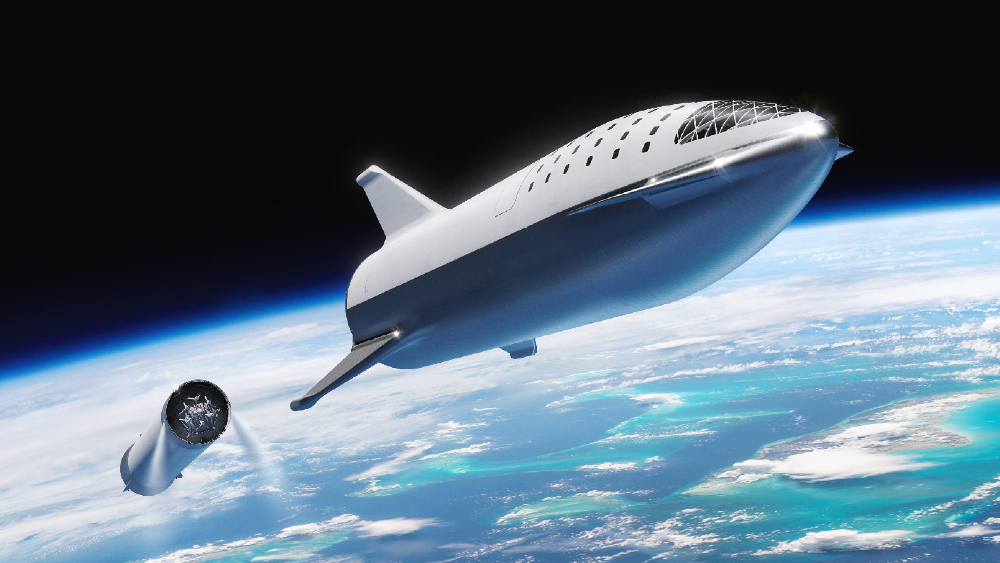
\includegraphics[width=\textwidth]{cover}
\end{figure}

\begin{abstract}
Spaceflight Dynamics is the science of spacecraft peformance, stability and control. It invloves he modeling of the changing position and orientation of a vehicle i.e. its trajectory via analysis of different ballistic and cellestial forces acting upon the six different degrees of freedom of a body. This project 
\end{abstract}
\setlength{\parindent}{0pt}
\newpage
\section{Introduction - Setting up the Groundwork}
\subsection{Particle Dynamics}
To understand the dynmamics of a spcaecraft, we must first set up the basis of our study and laydown the basic tools we shall be using to understand and analyse more complex problems. It all starts with Newtons Three Laws:
\begin{enumerate}

	\item A particle at rest remains in rest, and a partical in motion remains in motion, if the applied force is zero.
	\item The force on a particle equals the mass of the particle times its inertial acceleration.
	\item For every force applied, there is an equal and opposite reaction force.

\end{enumerate}

I need not go into the details and explanation of these, we all know their implications, nuances and caveats. Another important set of laws in our analysis are the ones layed down by Keppler. They are as follows:
\begin{enumerate}

	\item The orbit of a planet is an ellipse with the Sun at one of the two foci.
	\item A line segment joining a planet and the Sun sweeps out equal areas during equal intervals of time.
	\item The square of the orbital period of a planet is directly proportional to the cube of the semi-major axis of its orbit.

\end{enumerate}

 These laws were written down by Keppler after detail study and observation of our solar system, hence they describe the motion of planets in our solar system. However these are applicable to a much more genral case of the Two Body Problem. We shall see the same in that section. I shall now focus on building upon the math involved in applying these laws when in frames other than the inertial frame.

For starters, let us define the frame $i$ as the inertial frame and $s$ as the non-inertial frame. Now a vector $\mathbf{A}$ can be expressed in the inertial frame as:

\begin{displaymath} \mathbf{A^i} = A_{i1}i_1 + A_{i2}i_2 + A_{i3}i_3 \end{displaymath}
 
 where $i_1, i_2, i_3$ are a set of orthogonal basis vectors of the inertial frame. $\mathbf{A}$ can be represented in 
 the non - inertial frame as:

\begin{displaymath} \mathbf{A^s} = A_{s1}s_1 + A_{s2}i_2 + A_{s3}i_3 \end{displaymath}

where $s_1, s_2, s_3$ are a set of orthogonal basis vectors of the non-inertial frame. These two expressions are just representations of a vector in two different frames of reference, but the vector itself exists independent of any frame. The coordinate $A_i$ and $A_s$ are simply representations of the same vector. Both are related via a rotation matrix as given below. 

\begin{displaymath}
	\begin{bmatrix} A_{i1} \\ A_{i2} \\ A_{i3} \end{bmatrix} 
	=
	\begin{bmatrix}
	i_{1} \cdot s_{1} & i_{1} \cdot s_{2} & i_{1} \cdot s_{3}\\
	i_{2} \cdot s_{1} & i_{2} \cdot s_{2} & i_{2} \cdot s_{3}\\
	i_{3} \cdot s_{1} & i_{3} \cdot s_{2} & i_{3} \cdot s_{3}\\
	\end{bmatrix}
	\cdot
	\begin{bmatrix}
	A_{s1} \\ A_{s2} \\ A_{s3}
	\end{bmatrix}
\end{displaymath}
\begin{displaymath}	\mathbf{A^i} = R^{si}\mathbf{A^s} \end{displaymath}

Suppose the $\mathbf{A}$ vector represents distance. To calculate velocity and acceleration we must differentiate above equation. 

\begin{displaymath}
\frac{d}{dt}\mathbf{A^i} = \frac{d}{dt}(R^{si}\mathbf{A^s}) = \Dot{A^{si}}\mathbf{A^s} + R^{si}\Dot{\mathbf{A^s}}
\end{displaymath}

The rotation matrix when multiplied with its inverse or transpose, dissaperars. So we are left with:

\begin{displaymath}
\frac{{}^id}{dt}\mathbf{A} = \frac{{}^id}{dt}\mathbf{A} + R^{siT}\Dot{R^{si}}\mathbf{A^s}
\end{displaymath}

Now suppose the non-inertial frame is rotating with respect to the inertial frame with angular velocity $\mathbf{\omega^{si}}$. It can be shown that $R^{siT}\Dot{R^{si}} = \mathbf{\omega^{si}}$. As $\mathbf{A}$ can be any vector we can say that: 

\begin{displaymath}
\frac{{}^id}{dt}( ) = \frac{{}^id}{dt}( ) + \mathbf{\omega^{si}}\times()
\end{displaymath}

Similarly for acceleration, we must differentiate again. This gives us the following result:

\begin{displaymath}
\frac{{}^id^2}{dt^2}(\mathbf{R + r}) = \frac{{}^id^2}{dt^2}\mathbf{R} + \frac{{}^sd^2}{dt^2}\mathbf{r} + 2\mathbf{\omega^{si}}\times\frac{{}^sd}{dt}(\textbf{r}) + (\frac{{}^sd}{dt}\mathbf{\omega^{si}})\times\mathbf{r} + \mathbf{\omega^{si}}\times(\mathbf{\omega^{si}}\times\mathbf{r})
\end{displaymath}
Where $\mathbf{R}$ is the distance of the origin non-inertial frame from the origin of the inertial frame. What we have established so far along with a few high-school concepts shall make up our toolkit. Until now we have treated mass as dimensionless point partices, which is not the case in reality! We shall now see dynamics of systems if we consider the physical dimensions of the same.

\subsection{Rigid Body Dynamics}

A rigid body is generally a system with six degrees of freedom. Three degrees are related to the translational motion and the other three with rotational motion of the system. 

\subsubsection{Translational Dynamics}

On each particle in the system there will be internal and external forces acting upon it. Applying Netwton's second law to each particle in system and summing over all particles, we get:
\begin{displaymath}
\sum \mathbf{F_i} = \sum \mathbf{f_{int}} + \sum \mathbf{f_{ext}} = \sum m_i\mathbf{a_1}
\end{displaymath}


As the internal forces are equal and opposite in nature, the summation of internal forces over the entire system will amount to zero. We shall now define a new term called center of mass and its location $\mathbf{r_{cm}}$ is given as:
\begin{displaymath}
\mathbf{r_{cm}} = \frac{1}{M}\sum_{}^{} m_{i} \mathbf{r_{i}}
\end{displaymath}
 Combining the two equations we get:

 \begin{displaymath}
 \mathbf{F_e} = \sum \mathbf{f_{ext}} = \frac{d^2}{dt^2}\mathbf{r_{cm}}
 \end{displaymath}

This implies the center of mass behaves as if all the mass of the rigid body was concentrated there and all the external force was applied there.This covers the translational degrees of freedom. Note in the above formulation, if the system is a made up of a continous particle system, the summation is converted to an integral and $m_i$ to $dm$. Now to tackle the rotational degrees of freedom.

\subsubsection{Rotational Dynamics}

To analyse rotational dynamics, we must first encounter a quantity known as angular momentum($\mathbf{H}$). It is defined as follows:
\begin{displaymath}
\mathbf{H} = \int \mathbf{r} \times \mathbf{\omega} dm 
\end{displaymath}
Taking a referance frame tied to the body we get:
\begin{displaymath}
\mathbf{H} = \int \mathbf{r} \times (\mathbf{\omega^{bi}} \times \mathbf{r}) dm 
\end{displaymath}

where $\mathbf{\omega^{bi}}$ is the intertial angular velocity of the rigid body. We are now in a body frame of referance. Through splitting the terms into their components and further calculations we get:

\begin{displaymath}
\mathbf{H} = \bigintsss
	\begin{bmatrix}
	y^2 + z^2 & -yz &  -zx\\
	 -xy &  z^2 + x^2 &  -zy\\
	 -xy & -yz & x^2 + y^2\\
	\end{bmatrix}
	dm
	\begin{bmatrix}
	\omega_1\\
	\omega_2\\
	\omega_3\\
	\end{bmatrix}
\end{displaymath}

Here we define a new quantity called moment of inertia(I) given as:

\begin{displaymath}
	I = 
	\begin{bmatrix}
	\int(y^2 + z^2)dm & \int(-yz)dm & \int(-zx)dm\\
	\int(-xy)dm & \int(z^2 + x^2)dm & \int(-zy)dm\\
	\int(-xy)dm & \int(-yz)dm & \int(x^2 + y^2)dm\\
	\end{bmatrix}
\end{displaymath}

This gives us:

\begin{displaymath}
\mathbf{H} = I \mathbf{\omega^{bi}}
\end{displaymath}

Here \textbf{H} is not parallel to the angular velocity vector. This is not desirable. Thus we focus on a particular body frame called the pricipal axis frame. In this frame the moment of inertia tensor can be represented as a diagonal matrix. This frame can always be found by diagonalising the moment of inertia matrix via solving its charachteristic equation. We now move onto relating this with torque(\textbf{M}). Torque is generally given as:
\begin{displaymath}
\mathbf{M} = \frac{{}^id}{dt}\mathbf{H}
\end{displaymath}

Substituting the above equation for angular momentum and doing further calculations we get:

\begin{displaymath}
\mathbf{M} = I\dot{\mathbf{\omega^{bi}}} + \mathbf{\omega^{bi}}\times I \mathbf{\omega^{bi}}
\end{displaymath}

These give three non-linear first order differential equtions make up half of the equations required to fully describe the rotational motion of a system. To obtain the second half of the dynamics it is nicessary to introduce three angles specifying the orientation of the body with respect to the inertial frame and relate them to $\mathbf{\omega^{bi}}$. We shall do so using the classical euler angles: pitch, roll and yaw.

\begin{figure}[h]
	\centering
    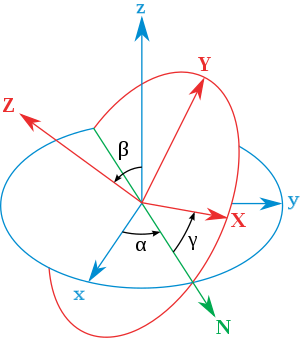
\includegraphics[width = 200px]{EulerAngles}
    \caption{Euler's Angles}
	\label{fig:euler}
\end{figure}

The Euler angles $\phi,\theta,\psi$ are shown in figure \ref{fig:euler}. The inertial frame is shown in blue while the body frame is in red. One goes from inertial frame to body frame by first rotating along the '\textbf{z}' axis by $\phi$ then about the node vector \textbf{N} by $\theta$ and finally about '\textbf{Z}' by $\psi$. The total rotation can be written as:

\begin{displaymath}
R^{ib} = R_3^{T}(\psi)R_1^{T}(\theta)R_1^{T}(\phi)
\end{displaymath}

Where $R_1$ and $R_3$ are elementary rotation matrices about the x and z axes repectively. Now from the figure we can write $\omega^{bi}$ as:

\begin{displaymath}
\mathbf{\omega^{bi}} = \dot{\phi}\mathbf{i_1} + \dot{\theta}\mathbf{n} + \dot{\psi}\mathbf{b_1}
\end{displaymath}

Upon further simplification, we can write $\omega^{bi}$ in its body frame components as:

\begin{gather*}
\omega_1 = \dot{\phi}sin{\theta}sin{\psi} + \dot{\theta}cos\psi\\
\omega_2 = \dot{\phi}sin{\theta}cos{\psi} - \dot{\theta}sin\psi\\
\omega_3 = \dot{\psi} + \dot{\phi}cos\theta
\end{gather*}

Also, via the differentiation rule and using the rotation matrix defined above, we can also get:

\begin{displaymath}
\dot{\mathbf{b_i}} = \mathbf{\omega^{bi}}\times\mathbf{b_i}
\end{displaymath}

These complete the necessary equations required to completely analyse the rotational motion of a system. There are other tequniques such as quaternion rotation that are alternatives to Euler's angles that are helpfull and advantageous in certin case senarios. Given this we are now ready to start further analysis of more complex systems. We shall start with the famous two body problem.

\newpage
\section{The Two Body Problem}
 The two body problem is the simplest gravitational problem, just two point masses orbiting under their mutual gravitational attraction. The problem is to describe the motion of both objects given initial conditions. Let there be two masses with distances from a inertial origin as shown in Figure \ref{fig:two}.

\begin{figure}[h]
	\centering
    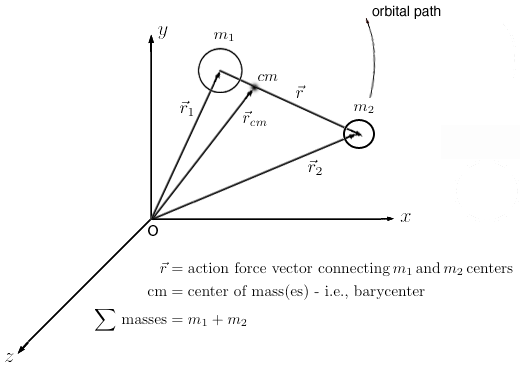
\includegraphics[width = 300px]{Twobodies}
    \caption{Two particles as seen from inertial frame}
    \label{fig:two}
\end{figure}

By equating gravitational forces on each object:
\begin{gather*}
m_1\mathbf{\ddot{R}_{1}} = \frac{-Gm_1m_2}{|\mathbf{R_2} - \mathbf{R_1}|^3}(\mathbf{R_1} - \mathbf{R_2})\\
m_2\mathbf{\ddot{R}_{2}} = \frac{-Gm_1m_2}{|\mathbf{R_2} - \mathbf{R_1}|^3}(\mathbf{R_2} - \mathbf{R_1})\\
\end{gather*}

Adding, we get:
\begin{displaymath}
m_1\mathbf{\ddot{R}_{1}}  + m_2\mathbf{\ddot{R}_{2}} = 0
\end{displaymath}

We also introduce another vector $\mathbf{R_{cm}}$ given as:
\begin{gather*}
\mathbf{R_{cm}} = \frac{m_1\mathbf{R_1}+m_2\mathbf{R_2}}{m_1 + m_2}
\end{gather*}
Hence, we get:
\begin{gather*}
\mathbf{\ddot{R}_{cm}} = 0 \\
\mathbf{R_{cm}} = \mathbf{R_{cm0}} + \mathbf{V_{cm0}}t
\end{gather*}

Where $\mathbf{R_{cm0}}$ and $\mathbf{V_{cm0}}$ are the position and velocity vectors of the center of mass at $t=0$ and are constants. From Figure 2, $\mathbf{r} = \mathbf{R_2} - \mathbf{R_1}$ is obvious. By using the initial force equations, we can see:

\begin{displaymath}
m_1m_2 \mathbf{\ddot{r}} = \frac{-Gm_1m_2(m_1+m_2)}{r^3}\mathbf{r}
\end{displaymath}

Writing $\mu = G(m_1+m_2)$, we get:
\begin{displaymath}
\mathbf{\ddot{r}}  = \frac{-\mu\mathbf{r}}{r^3}
\end{displaymath}

This equation describes relative motion. Taking dot product of above equation with $\mathbf{\dot{r}}$ and further simplification, we get:

\begin{gather*}
\begin{split}
\frac{d}{dt}\frac{1}{2}\dot{r}^2 & = - \frac{\mu}{r^2}\dot{r}\\
								& = - \frac{d}{dt}\Big(-\frac{\mu}{r}\Big)
\end{split}
\end{gather*}

Substituting,
\begin{displaymath}
V = -\frac{\mu}{r}
\end{displaymath}

Where V is the potential energy per unit mass, we get:
\begin{displaymath}
\mathcal{E} = \frac{1}{2}v^2 + V
\end{displaymath}

Hence the total energy is conserved. Note, here $\mathcal{E}$ represents the total energy per unit mass and not the entire mechanical energy. This is beneficial in some case senarios and can be easier to work with. We shall now attempt to find the orbit equation. To do this, take cross product with radius vector $\mathbf{r}$ on both sides of relative motion equation. The R.H.S goes to zero as cross product of vector with itself is zero. Integrating we get:

\begin{displaymath}
\mathbf{r}\times\mathbf{\dot{r}} = \mathbf{H}
\end{displaymath}

Here \textbf{H} is the angular momentum per unit mass which is again a constant. Here \textbf{H} is also equal to twice the rate of description of the position vector of $m_2$ with respect to $m_1$. This proves Keppler's second law. Now to solve the initial differntial equation, take right hand cross product of relative motion equation with \textbf{H}. Upon solving further, we get:

\begin{displaymath}
{r} = \frac{{H^2}/\mu}{1 + e\:cos\nu}
\end{displaymath}

Where $\mathbf{e}$ is a integration constant vector. It is termed as the \textit{eccentricity vector} and its scalar magnitude is simply the eccentricity of the orbit while direction is from the focus to the periapsis. The angle $\nu$ is the angle between the position vector($\mathbf{r}$) and the eccentricity vector and is termed as the \textit{true anomaly}. The above equation is the polar form of a conic section with the origin as one of the focii. If $e < 1$, the orbit is elliptical, $e = 1$ implies a parabolic orbit and $e > 1$ implies a hyperbolic orbit. We shall see indepth analysis of these in a later section. Now, the two body problem was completely solvable and we got a neat result. But real life has cerainly more than just two bodies. Let us now look into the N Body Problem.

\subsection{The N Body Problem}

We shall start by employing a route similar to that of the two body problem. Define $ \mathbf{r_{ij}} = \mathbf{R_{j}} - \mathbf{R_{i}}$. Applying Gravitational Law on each object:

\begin{displaymath}
m_i\mathbf{\ddot{r}_i} = \sum_{j \neq i}^{N} \frac{Gm_im_j}{r_{ij}^3}\mathbf{r_{ij}}
\end{displaymath}

When we sum all the above equations, the R.H.S goes to zero due to Newton's third law. All forces are equal and opposite and cancel each other out in the summation. We get:

\begin{displaymath}
\sum_{i=1}^{N} m_i\mathbf{\ddot{r}_i} = 0
\end{displaymath}

This leads us to:

\begin{gather*}
M\mathbf{\ddot{r}_{cm}} = 0\\
\mathbf{r_{cm}}(t) = \mathbf{r_{cm0}} + \mathbf{V_{cm0}}t
\end{gather*}

Following the steps taken in the two body problems with a few minor modifications, we can obtain the following quantities:

\begin{gather*}
\mathbf{H} = \sum_{i=1}^{N} m_i\mathbf{r_i}\times\mathbf{\dot{r}_i}\\
V = -\frac{1}{2}\sum_{i=1}^{N}\sum_{j \neq i}^{N}\frac{Gm_im_j}{r_{ij}}\\
\mathcal{E} = \sum_{i=1}^{N}\frac{1}{2}m_i\mathbf{\dot{r}_i}\cdot\mathbf{\dot{r}_i} + V
\end{gather*}

This all we can absolutely determine for a N-Body system. Further solutions cannot be obtained "absolutely" and through various mathematical techniques and approximations, we can obtain models that nearly replicate real life systems. With this done, we shall temporarily shift our focus and look into the aerodynamic aspects of rockets.

\newpage

\section{A Few Problems}
\textit{Q1. Show that a object in a hyperbolic trajectory as seen from the other object arrives at $r = \infty $ with residual speed:}
\[
	v_\infty = \sqrt{-\frac{\mu}{a}} = \sqrt{2\mathcal{E}}
\]

A1. We know that total energy per object is conserved. So let us find the total energy per object at the perigee. First we need to find the velocity of the object at the perigee. At the perigee of a hyperbola, the radius vector and velocity vector are perpendicular:
\begin{gather*}
	\mathbf{H} = \mathbf{r\times v}\\
	\implies H_p = r_pv_p
\end{gather*}
Putting this in orbit equation:

\begin{gather*}
	{r} = \frac{{H^2}/\mu}{1 + e\:cos\nu}
	\implies v_p^2 = \mu \frac{1 + e\:cos\nu}{r_p}
\end{gather*}

As $a$ is a negative quantity(As everything is defined with respect to the eccentricity vector), $r = a + ae$ and $cos\nu = 1$. Thus we get:
\begin{gather*}
	v_p^2 = \frac{\mu}{a}
\end{gather*}
Putting this in the energy equation.
\begin{gather*}
\begin{split}
	\mathcal{E} &= \frac{1}{2}\frac{\mu}{a} - \frac{\mu}{a}\\
	&= - \frac{\mu}{2a}
\end{split}
\end{gather*}

We know that this will remain the net energy per object when the object reaches apogee, which in a hyperbolic trajectory is $\infty$.
\begin{gather*}
	\mathcal{E} = \frac{1}{2}v_\infty^2 - 0\\
	\begin{split}
	\implies v_\infty &= \sqrt{2\mathcal{E}}\\
	&= \sqrt{-\frac{\mu}{a}}
	\end{split}
\end{gather*}

Hence Proved.
\newpage
\textit{Q2. Halley's Commet passed perihelion on Feburary 9, 1986. It has a semi-major axis a = 17.9564 AU and e = 0.967298. Find the scalar radius as a function of time and the Time period.}\newline

A2. Following simillar working as the previous question, we get $\mathcal{E} = -\frac{\mu}{2a} $. Putting that back into the energy equation for and given time:

\begin{gather*}
	-\frac{\mu}{2a} = \frac{1}{2}v^2 - \frac{\mu}{r}\\
	\implies \frac{dr}{dt} = \sqrt{\mu(\frac{2}{r}-\frac{1}{a})}
\end{gather*}

Integrating that we get,
\[
	t - t_0 = \frac{(\pi+2)a^{\frac{3}{2}}}{2\sqrt{\mu}} - \frac{2a^{\frac{3}{2}}\sqrt{\mu}\arctan(\sqrt{\frac{2\mu a -\mu r}{\mu r}}) + \sqrt{ar(2\mu a -\mu r)}}{\mu}
\]
Where $t_0$ is the time at which the the comet is at perigee. Putting $r=a$ we get $T \approx 75$yrs.
\newpage
\section{Revised Timeline}

Week 3 (27/4 - 3/5): Dive deeper into orbital mechanics, starting with the various conic orbitals and then the orbital elements. Then a brief overview of orbital transfer movements and payload deployment.\\

Week 4 (4/5 - 10/5): Start looking into the aerodynamic aspects of the rocket and studying the space environment. Underlying physics and mathematical treatement of the same. \\

Week 5 (11/5 - 17/5): Look into planetary fly-bys, gravitational turn trajectories, and interplanetary trajectories.\\

Week 6 (18/5 - 24/5): Learning about the propulsion techniques employed, launch se- quences, the problems faced and how they are overcome. The multistage and single stage rocket concepts. Difference and benefits of bell thrusters and aerospikes.\\

Week 7 (25/5 - 31/5): Learn about re-entry dynamics. plotting re-entry trajectories( top- ics like polynomial descent gradient), the physics and maths that go behind re-entries.\\

Week 8 (4/5 - 9/5): Analysis of SpaceX’s booster landings for more recent developments and to gain better understanding.\\

\end{document}






























